%  LaTeX support: latex@mdpi.com
%=================================================================
\documentclass[article,submit,pdftex,moreauthors]{Definitions/mdpi}

\firstpage{1}
\makeatletter
\setcounter{page}{\@firstpage}
\makeatother
\pubvolume{1}
\issuenum{1}
\articlenumber{0}
\pubyear{2026}
\copyrightyear{2026}
\datereceived{ }
\dateaccepted{ }
\datepublished{ }

%=================================================================
\Title{Data-Efficient Learning from EMG Signals for Hand Gesture Recognition}


\Author{Mohammed Mizan $^{1}$ and Prof. Yassine Bouteraa $^{2}$}

\AuthorNames{Mohammed Mizan Alanazi and Yassine Bouteraa}

\address{%
$^{1}$ \quad Department of Computer Science, Prince Sattam bin Abdulaziz University, Al-Kharj, Saudi Arabia; 446540203@std.psau.edu.sa\\
$^{2}$ \quad Department of Computer Science, Prince Sattam bin Abdulaziz University, Al-Kharj, Saudi Arabia; y.bouteraa@psau.edu.sa}


\abstract{Surface electromyography (sEMG) provides a way that's allow us to detect the human gesture movement in purpose to use for robotics control. However,the differences between subjects is a big difficulty since the same gesture might change between individuals. This paper goals is to establish a method can accurately classify the gestures which will help us transfer it to robotics. Using the NinaPro DB2 dataset with 40 subjects and five gesture classes, a preprocessing pipeline applied 3 different processes. A ResCNN with three residual blocks (647K parameters) was trained on 60 subjects with adaptive mixup and Gaussian noise augmentation, then evaluated on 10 held-out test subjects. Using the window level predictions, the model achieved 69.87\% accuracy and a macro F1 score of 0.68. While using hard majority voting the model achieved 89.78\% accuracy and macro F1 of 0.83; also, soft voting achieved close results (89.37\%, macro F1 of 0.83). These results shows that simple voting strategies can achieved better results since it less sensitive to noise, outliers, and subjects motions compare to window-level predictions.}

\keyword{EMG; gesture recognition; deep learning; residual networks; majority voting; CNN}

%%%%%%%%%%%%%%%%%%%%%%%%%%%%%%%%%%%%%%%%%%
\begin{document}


%%%%%%%%%%%%%%%%%%%%%%%%%%%%%%%%%%%%%%%%%%

\section{Introduction}

Surface electromyography (sEMG) is useful in purpose to control robotics and prosthetic because it measure and record electrical activity signals from the muscles during regular contractions. But even with this converting sEMG signals into gesture command used by robotics still difficult because the same motion or gesture can differ significantly from individual to another due many causes like muscle structure, electrode location, and exhaustion \citep{zou2021transfer}.

Deep learning, especially CNN help to better recognition of sEMG gestures by learning features hierarchically from the signals raw data, eliminate our need for handcrafted feature engineering \citep{Li2021gesture}. Zero shot cross user performance has been successful with large scale and different users sEMG datasets, but these datasets are expensive and unavailable to individual researchers, and many methods for small datasets still require per-subject changes that affect usability\citep{eddy2024big}.


This paper aim to determine if a compact 1D ResCNN (a deep convolutional neural network that employs residual connections) combined with segment, level majority voting can yield state-of-the-art accuracies when only trained on data from a few (in this scenario 13) individuals and provided a moderately sized public dataset, we propose a method where a simple and computationally efficient neural network that requires 647k  parameters can obtain meaningful cross - subject generalization and that taking the majority of predictions computed at segment level can notably improve prediction precision, compared with when prediction is obtained only at window level.

%%%%%%%%%%%%%%%%%%%%%%%%%%%%%%%%%%%%%%%%%%
\section{Related Work}

\subsection{CNN-Based EMG Gesture Recognition}

CNNs are overwhelmingly the dominant method today for sEMG - based gesture recognition. \cite{bo2021hand} proposed a CNN model for hand gestures using raw sEMG signals. This research shows that deep neural networks are able to extract relevant temporal and spatial features on their own, without requiring time - consuming manual feature extraction. \cite{morozumi2021fundamental} use the discrete wavelet transform (DWT) for sEMG analysis, showing that frequency - domain decomposition is an effective approach for identifying various muscle activity patterns from the raw sEMG signals.

\subsection{Few-Shot and Transfer Learning Approaches}

The cross subject generalization problem has been addressed using few shot and transfer learning techniques. \cite{rahimian2021fs} Developed meta learning strategy to quickly adapt to new individuals with few data, moreover \citep{Rahimian2021trustworthy} integrate attention mechanisms and temporal convolution. \cite{Tam2022siamese}, employed CNN architectures to embed gestures on low resource systems and lessen training data demands. \cite{islam2024surface} merged a compact All ConvNet architecture with transfer learning to improve both inter session and inter subject performance. A prototype adaptation method called EMG - Adapt, described in \cite{lee2026few}, demonstrated top tier cross user generalization across public EMG datasets, including five widely used ones.

\subsection{Sequence-Level Aggregation}

Aggregating window-level predictions into sequence-level decisions has proven effective in related domains. \cite{dallel2022sliding} combined sliding windows with majority voting for online human action recognition, demonstrating that voting mechanisms substantially improve stream-based classification accuracy. This approach inspired the segment-level voting method used in the present work.

Despite these advances, many few-shot frameworks add architectural complexity that makes fair benchmarking difficult. The present work demonstrates that a simple residual CNN with majority voting can achieve strong cross-subject performance without meta-learning or domain adaptation.

Combining window level predictions and sequence level has prove its effective in the related domain. \cite{dallel2022sliding} combine sliding windows with majority voting to recognize online human action. show that add vote evaluation can improve performance. This inspired the way that segments vote in this paper. The methods in a few shot setting tend to add complex architecture, which can make it difficult to compare on fair grounds. We show that a simple residual CNN plus majority vote can lead to high accuracy across subjects, even in the absence of meta learning or domain adaptation. 

%%%%%%%%%%%%%%%%%%%%%%%%%%%%%%%%%%%%%%%%%%
\section{Methodology}

\subsection{Dataset and Subject Split}

This paper use the NinaPro DB2 dataset \citep{Atzori2014emg}, containing 12-channel sEMG recordings from 40 healthy subjects at 2000Hz. Five gestures were selected: Rest (0), Fist (1), Large Diameter Grasp (2), Wrist Pronation (3), and Tripod Grasp (4). Subjects were splited with seed 123 into 24 training, 6 validation, and 10 test subjects. these splits insure that every subject only appear in the split belong to it.

\subsection{Preprocessing}

To prevent data leakage each subject passed to the following preprocessing:
\begin{enumerate}
\item \textbf{Bandpass filtering:} using a fourth order Butterworth filter ($20-450$ Hz) with zero phase distortion (\texttt{sosfiltfilt}).
\item \textbf{Notch filtering:} Zero phase IIR notch filter at $50$ Hz ($Q=30$, \texttt{filtfilt}).
\item \textbf{Z-score normalization:} using a subject's $\mu$ and $\sigma$:
\begin{linenomath}
\begin{equation}
x_{\text{norm}} = \frac{x - \mu_{\text{subject}}}{\sigma_{\text{subject}} + \epsilon},\quad \epsilon = 10^{-8}
\end{equation}
\end{linenomath}
\end{enumerate}

\begin{figure}[H]
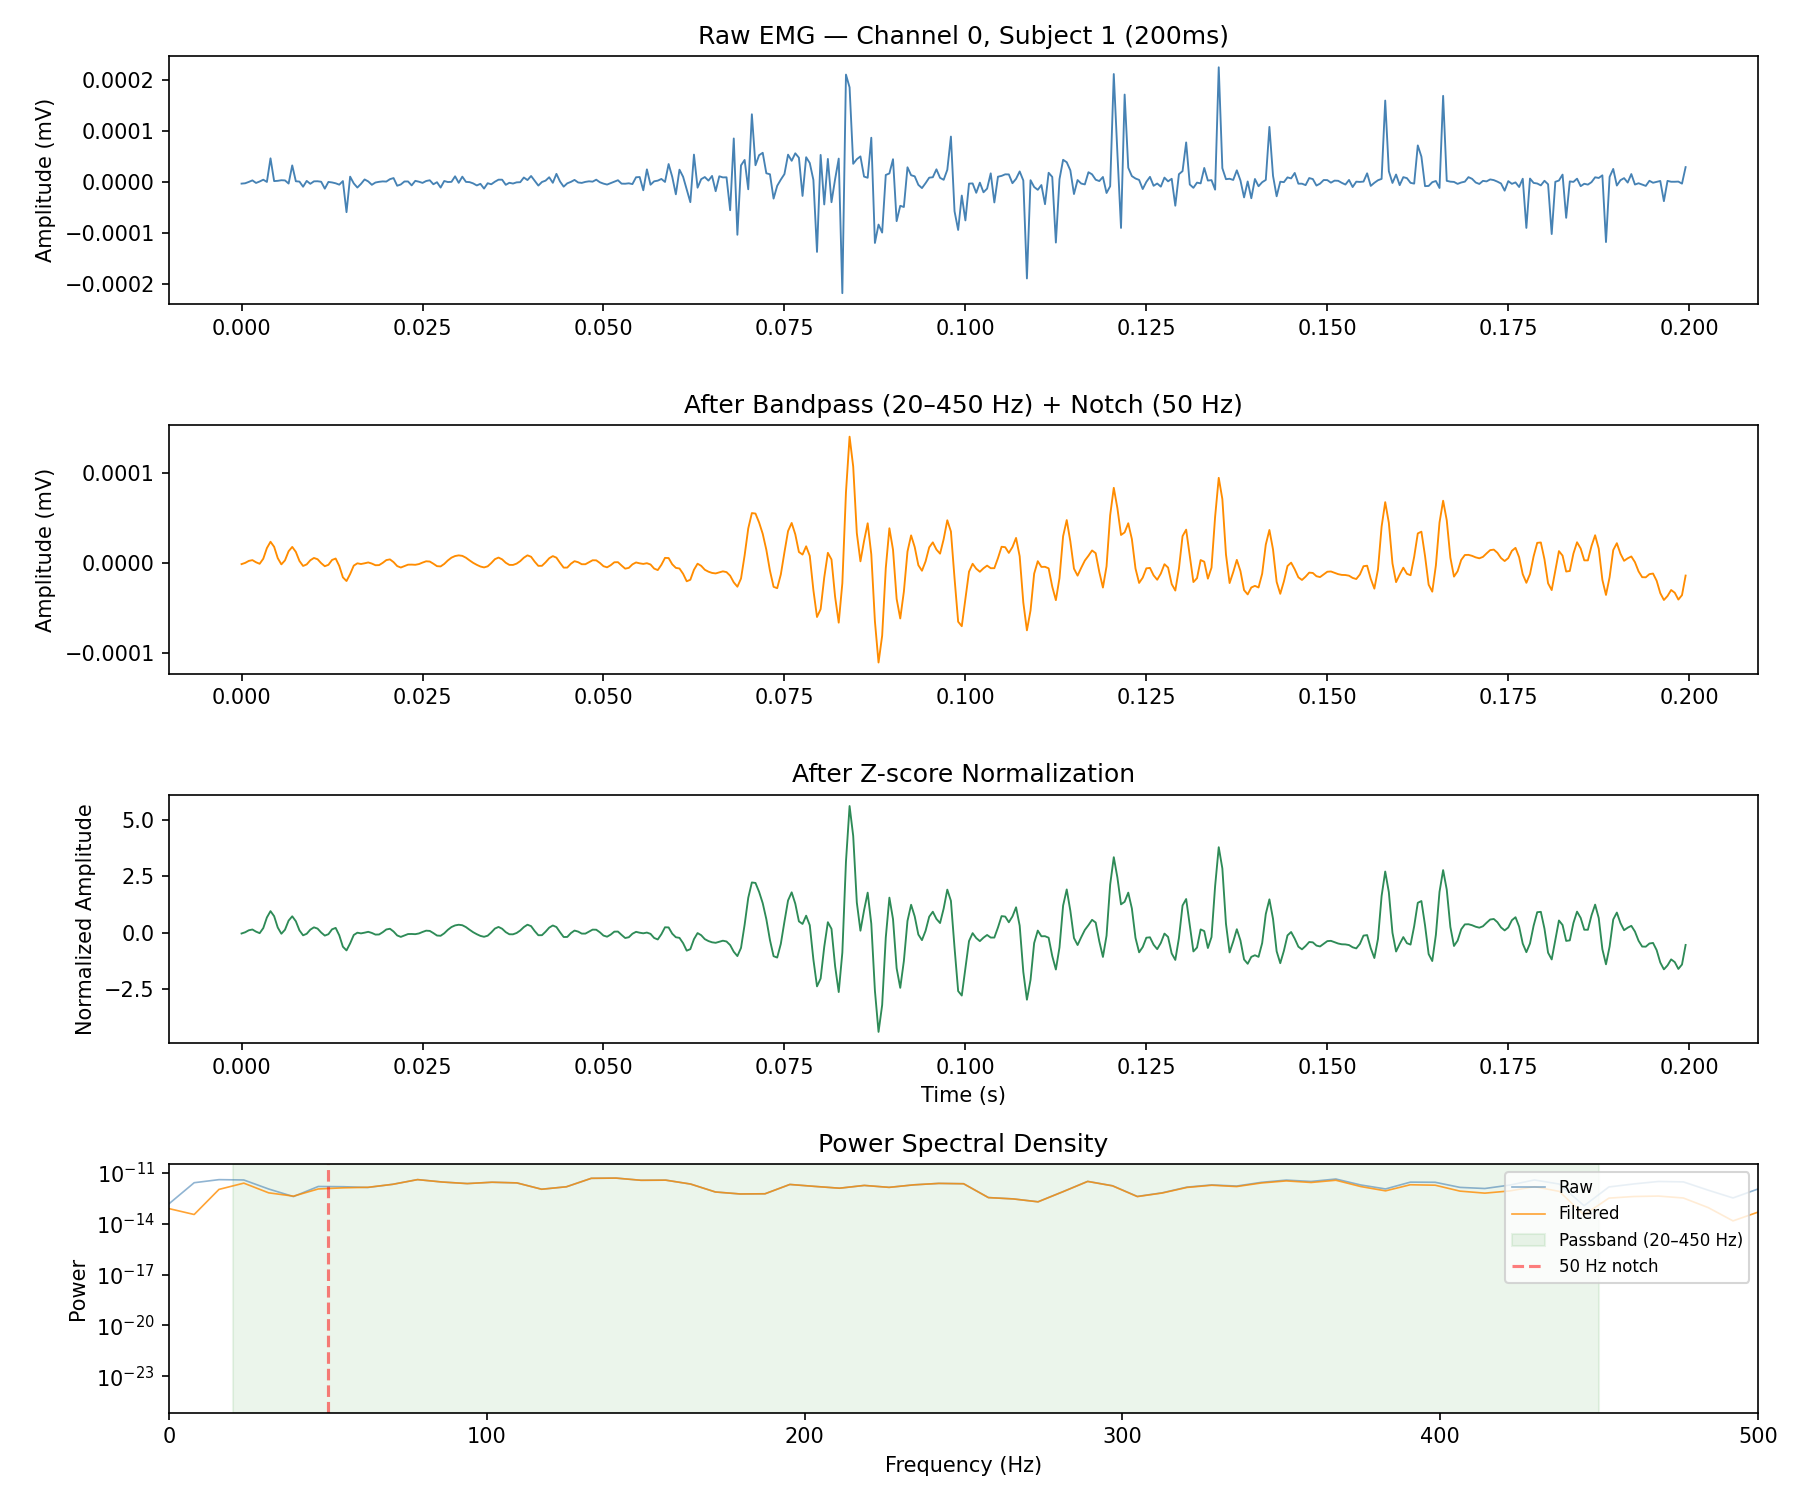
\includegraphics[width=0.90\textwidth]{figures/preprocessing_comparison.png}
\caption{Preprocessing pipeline stages (Subject 1, channel 0).\label{fig:preprocessing}}
\end{figure}

The windows were extracted of 200 samples (100ms) with step 50 (75\% overlap). Only 5 gestures included and other gestures excluded in each window. this process generate 141,543 training, 35,947 validation, and 62,087 test windows.

\begin{figure}[H]
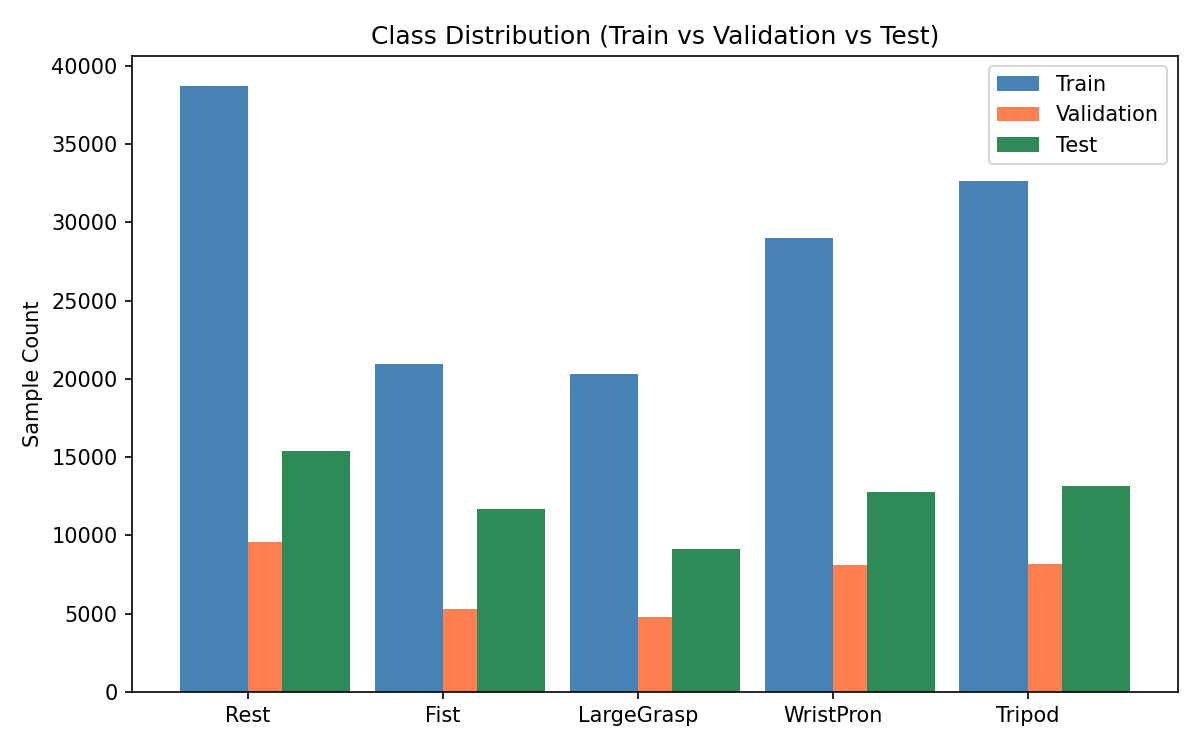
\includegraphics[width=0.95\textwidth]{figures/class_distribution.png}
\caption{Class distribution by data split.\label{fig:classdist}}
\end{figure}

\subsection{Model Architecture}

\begin{table}[H]
	\caption{1D ResCNN architecture (646,853 parameters).\label{tab:rescnn}}
	\begin{tabular}{ccc}
		\toprule
		\textbf{Stage} & \textbf{Layer} & \textbf{Channels} \\
		\midrule
		Stem & Conv1d$\to$BN$\to$GELU$\to$MaxPool1d(2) & 12$\to$64, k=15 \\
		ResBlock$_1$ & [Conv1d$\to$BN$\to$GELU]$_{\times2}\to$shortcut$\to$MaxPool1d(2) & 64$\to$64, k=15 \\
		ResBlock$_2$ & [Conv1d$\to$BN$\to$GELU]$_{\times2}\to$shortcut$\to$MaxPool1d(2) & 64$\to$128, k=7 \\
		ResBlock$_3$ & [Conv1d$\to$BN$\to$GELU]$_{\times2}\to$shortcut$\to$MaxPool1d(2) & 128$\to$256, k=3 \\
		Head & AdaptiveAvgPool1d(1)$\to$Dropout(0.5)$\to$Linear & 256$\to$5 \\
		\bottomrule
	\end{tabular}
\end{table}



\subsection{Training and Augmentation}

Training use AdamW optimizer (learning rate = $2 \times 10^{-3}$, weight decay = $3 \times 10^{-3}$) with label smoothing (0.1), ReduceLROnPlateau strategy (factor = 0.5, patience = 10, minimum learning rate = $10^{-6}$), gradient clipping (maximum L2 norm = 1.0) and batch size 256 was employed during the training. Weighted random sampling was used, where $w_i = 1 / C_{y_i}$ is applied to sample instances, for addressing the class imbalance. Training stopped after 78 epochs (max=100 and patience=30 ). Two data augmentation techniques were used, Additive Gaussian noise ($ \sigma=0.03$) and Adaptive MixUp ($\alpha = 0.25$ from epoch 1 to 25, $\alpha = 0.05$ from epoch 26 to 49 and no MixUp from epoch 50).

\subsection{Majority Voting}

Gesture predictions  produced by combining window predictions within gesture segments, Segments with gaps exceeding $2\times\text{windows\_step}$ or fewer than three windows were excluded, Which enhance the precision of the decision. Two voting methods were used:
\begin{linenomath}
\begin{equation}
\text{Hard Vote: } \hat{y}_{\text{gesture}} = \underset{c \in \{0,1,2,3,4\}}{\arg\max} \sum_{i=1}^{N} \mathbb{1}[y_i = c]
\end{equation}
\begin{equation}
\text{Soft Vote: } \hat{y}_{\text{gesture}} = \underset{c \in \{0,1,2,3,4\}}{\arg\max} \sum_{i=1}^{N} P(y_i = c)
\end{equation}
\end{linenomath}
where $N$ is the number of windows in that continuous gesture segment.

\subsection{Evaluation Metrics}

Window level and segment level performance were evaluated using accuracy and F1 score. For each class $c$:
\begin{linenomath}
\begin{equation}
\text{Precision}_c = \frac{TP_c}{TP_c + FP_c}
\end{equation}
\begin{equation}
\text{Recall}_c = \frac{TP_c}{TP_c + FN_c}
\end{equation}
\begin{equation}
F1_c = 2 \cdot \frac{\text{Precision}_c \cdot \text{Recall}_c}{\text{Precision}_c + \text{Recall}_c}
\end{equation}
\begin{equation}
\text{Accuracy} = \frac{\text{Correct Predictions}}{\text{Total Predictions}}
\end{equation}

\end{linenomath}

\subsection{Hyperparameters}

\begin{table}[H]
\caption{Training hyperparameters.\label{tab:hyperparams}}
\begin{tabularx}{\textwidth}{ll}
\toprule
\textbf{Parameter} & \textbf{Value} \\
\midrule
Model Parameters & 647K \\
Window size / step & 200 / 50 \\
Optimizer & AdamW \\
Learning Rate & $2 \times 10^{-3}$ \\
Scheduler & ReduceLROnPlateau \\
Loss & Cross-entropy \\
Dropout & 0.5 \\
Mixup & Adaptive ($\alpha = 0.25$, 0.05, off at epoch 50) \\
Batch size & 256 \\
Max epochs / early stop patience & 100 / 30 \\
\bottomrule
\end{tabularx}
\end{table}

%%%%%%%%%%%%%%%%%%%%%%%%%%%%%%%%%%%%%%%%%%
\section{Experimental Results}

\subsection{Training Dynamics}

The best validation accuracy of 75.28\% was achieved at epoch 49 (macro F1 0.74), early stopping happened at epoch 78 (Figure~\ref{fig:curves}).

\begin{figure}[H]
 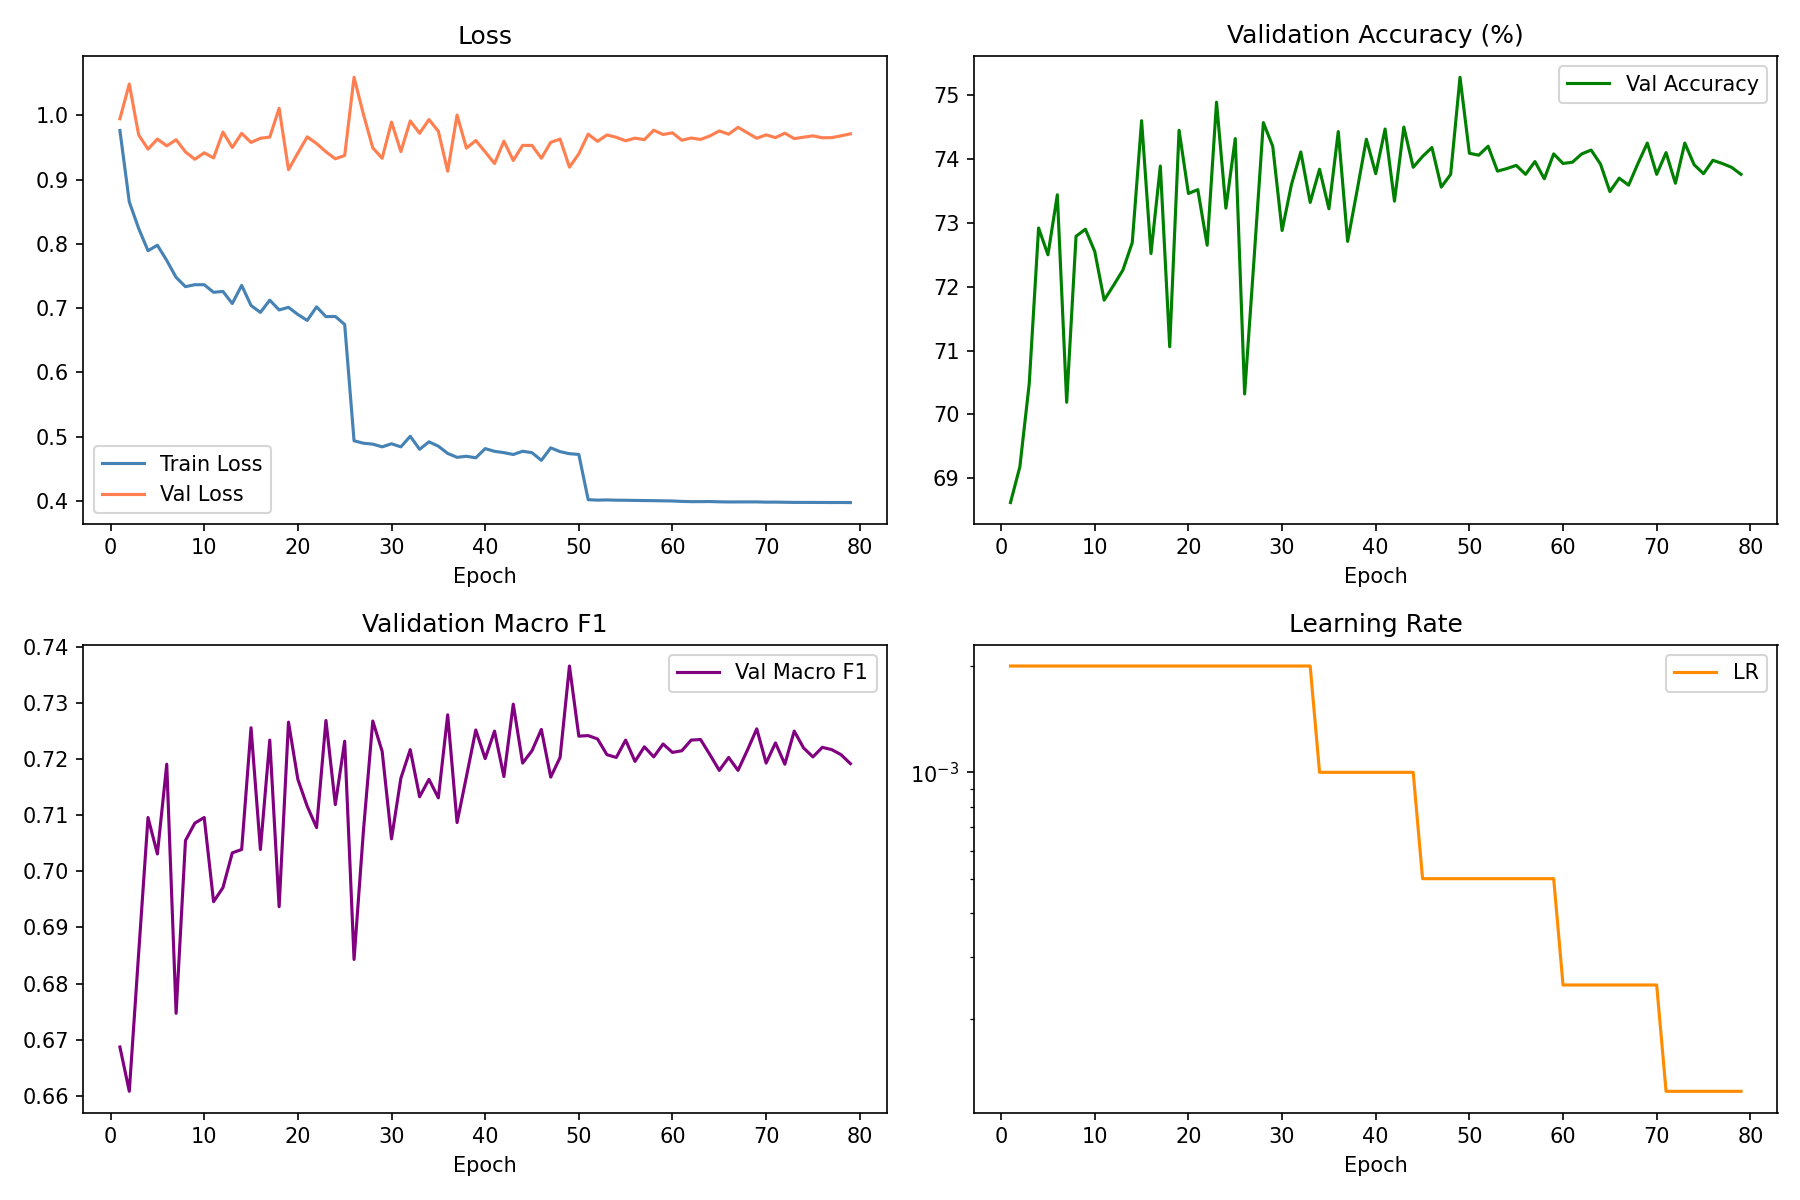
\includegraphics[width=0.95\textwidth]{figures/training_curves.png}
\caption{Training and validation metrics over epochs.\label{fig:curves}}
\end{figure}

\subsection{Window-Level Results}

Window level evaluation results 69.87\% accuracy and F1 score of 0.68 (Table~\ref{tab:window_results}, Figure~\ref{fig:confusion}).

\begin{table}[H]
\caption{Per-class window-level classification results ($n = 62,\!087$).\label{tab:window_results}}
\begin{tabularx}{\textwidth}{lcccc}
\toprule
\textbf{Gesture} & \textbf{Precision} & \textbf{Recall} & \textbf{F1} & \textbf{Support} \\
\midrule
Rest        & 0.99 & 1.00 & 1.00 & 15,391 \\
Fist        & 0.72 & 0.51 & 0.60 & 11,690 \\
LargeGrasp  & 0.66 & 0.72 & 0.69 & 9,114 \\
WristPron   & 0.58 & 0.44 & 0.50 & 12,756 \\
Tripod      & 0.53 & 0.75 & 0.62 & 13,136 \\
\midrule
Macro Avg   & 0.70 & 0.68 & 0.68 & -- \\
Weighted Avg & 0.71 & 0.70 & 0.69 & -- \\
\bottomrule
\end{tabularx}
\end{table}

\begin{figure}[H]
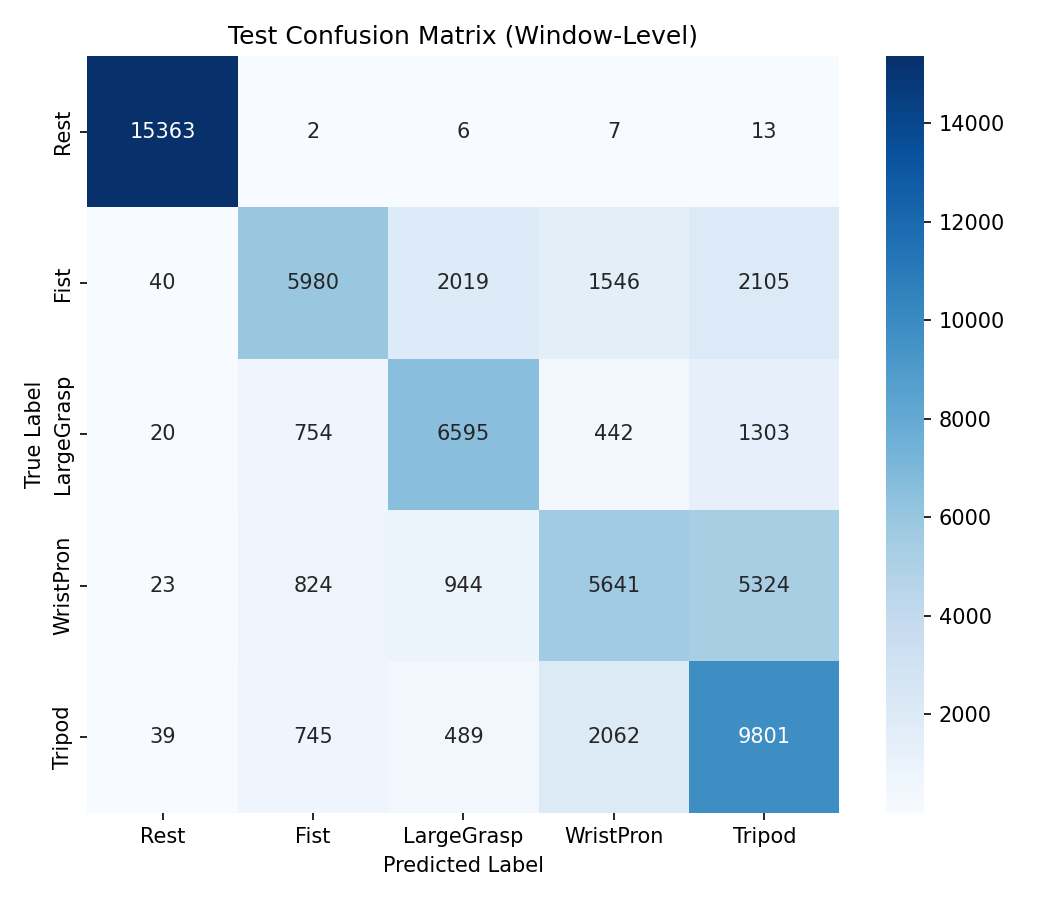
\includegraphics[width=0.95\textwidth]{figures/confusion_matrix.png}
\caption{Window-level confusion matrix on the test set.\label{fig:confusion}}
\end{figure}

\subsection{Segment-Level Results}

Hard voting achieved 89.78\% accuracy (macro F1 0.83), and soft voting achieve 89.37\% (macro F1 0.83) (Table~\ref{tab:voting}). Per-class segment accuracies: Rest 100.00\%, Fist 83.33\%, LargeGrasp 98.33\%, WristPron 53.33\%, and Tripod 81.67\% (Figure~\ref{fig:hardvote_cm}).

\begin{table}[H]
\caption{Window vs.\ segment-level performance.\label{tab:voting}}
\begin{tabularx}{\textwidth}{lccc}
\toprule
\textbf{Metric} & \textbf{Window} & \textbf{Hard Vote} & \textbf{Soft Vote} \\
\midrule
Accuracy (\%) & 69.87 & 89.78 & 89.37 \\
Macro F1      & 0.68 & 0.83 & 0.83 \\
\bottomrule
\end{tabularx}
\end{table}

\begin{figure}[H]
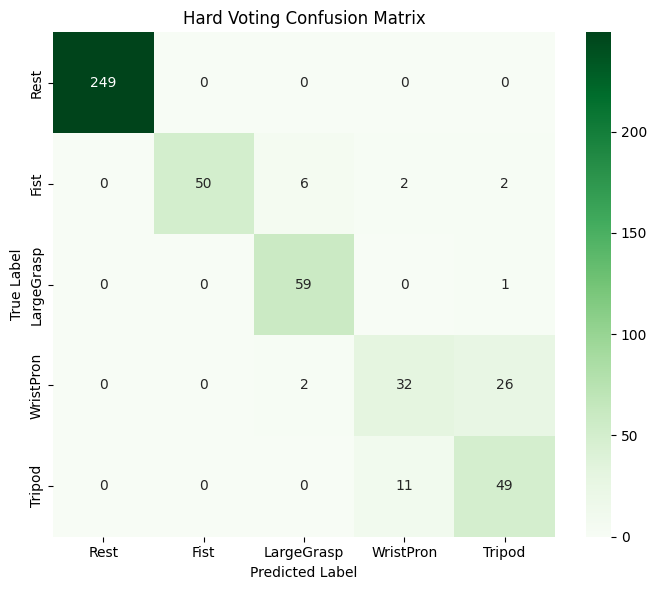
\includegraphics[width=0.95\textwidth]{figures/hard_voting_confusion_matrix.png}
\caption{Hard voting confusion matrix.\label{fig:hardvote_cm}}
\end{figure}

\subsection{Per-Subject and Feature Analysis}

Figure~\ref{fig:persubject} shows per-subject test accuracy. Subject 2 get above 0.95 for all classes, Where subjects 14 and 21 scored below 0.30 on Wrist Pronation and Tripod. The t-SNE   (Figure~\ref{fig:tsne}) shows Rest as a cluster, while Wrist Pronation and Tripod features heavily overlap.

\begin{figure}[H]
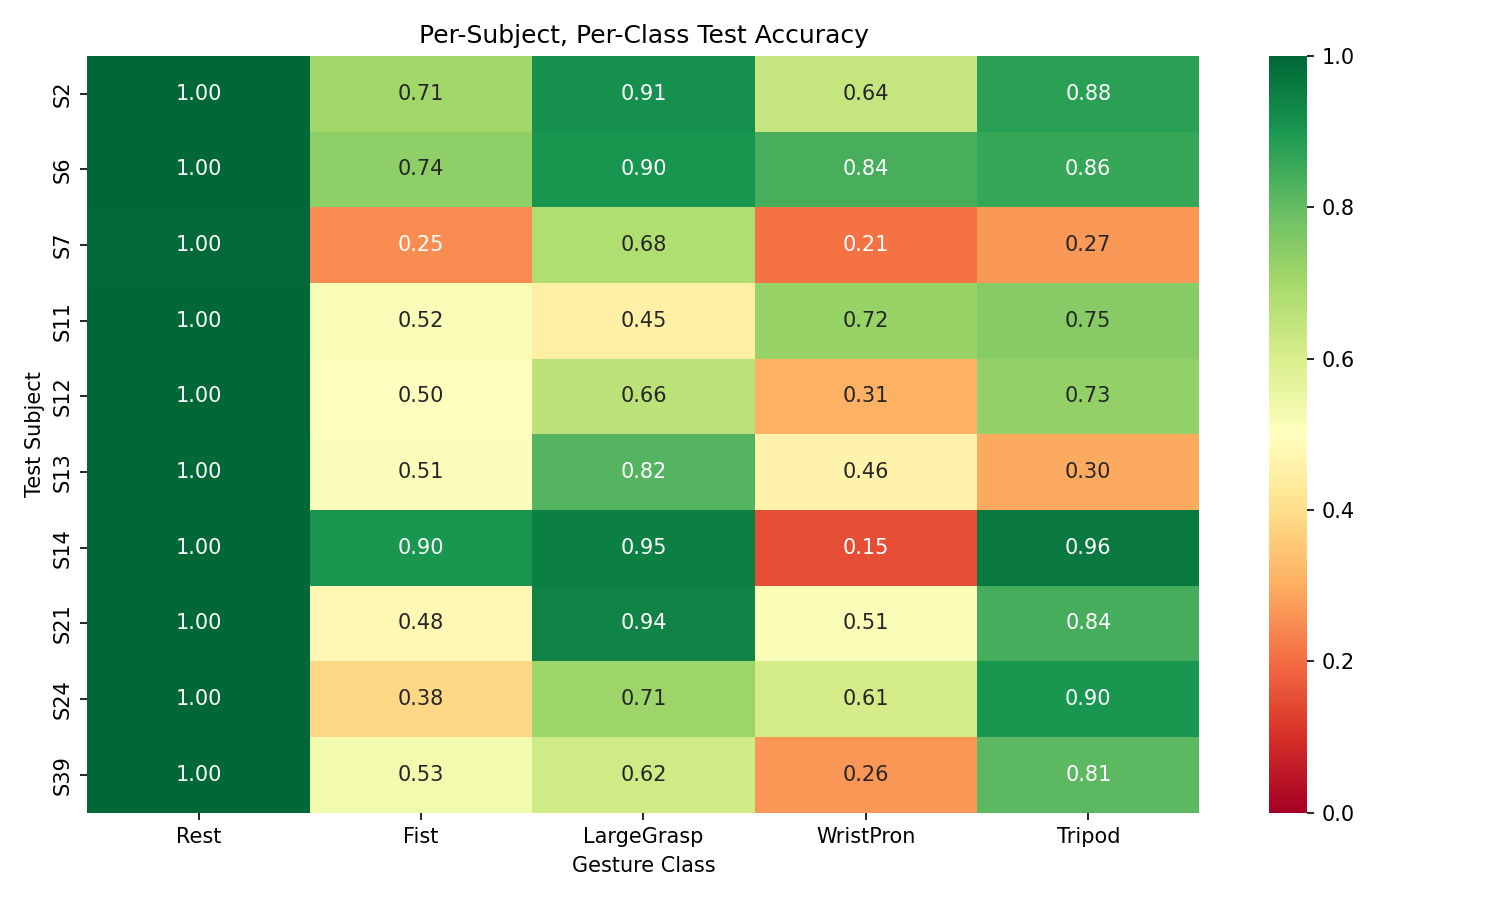
\includegraphics[width=0.95\textwidth]{figures/per_subject_accuracy.png}
\caption{Per-subject per-class accuracy heatmap.\label{fig:persubject}}
\end{figure}

\begin{figure}[H]
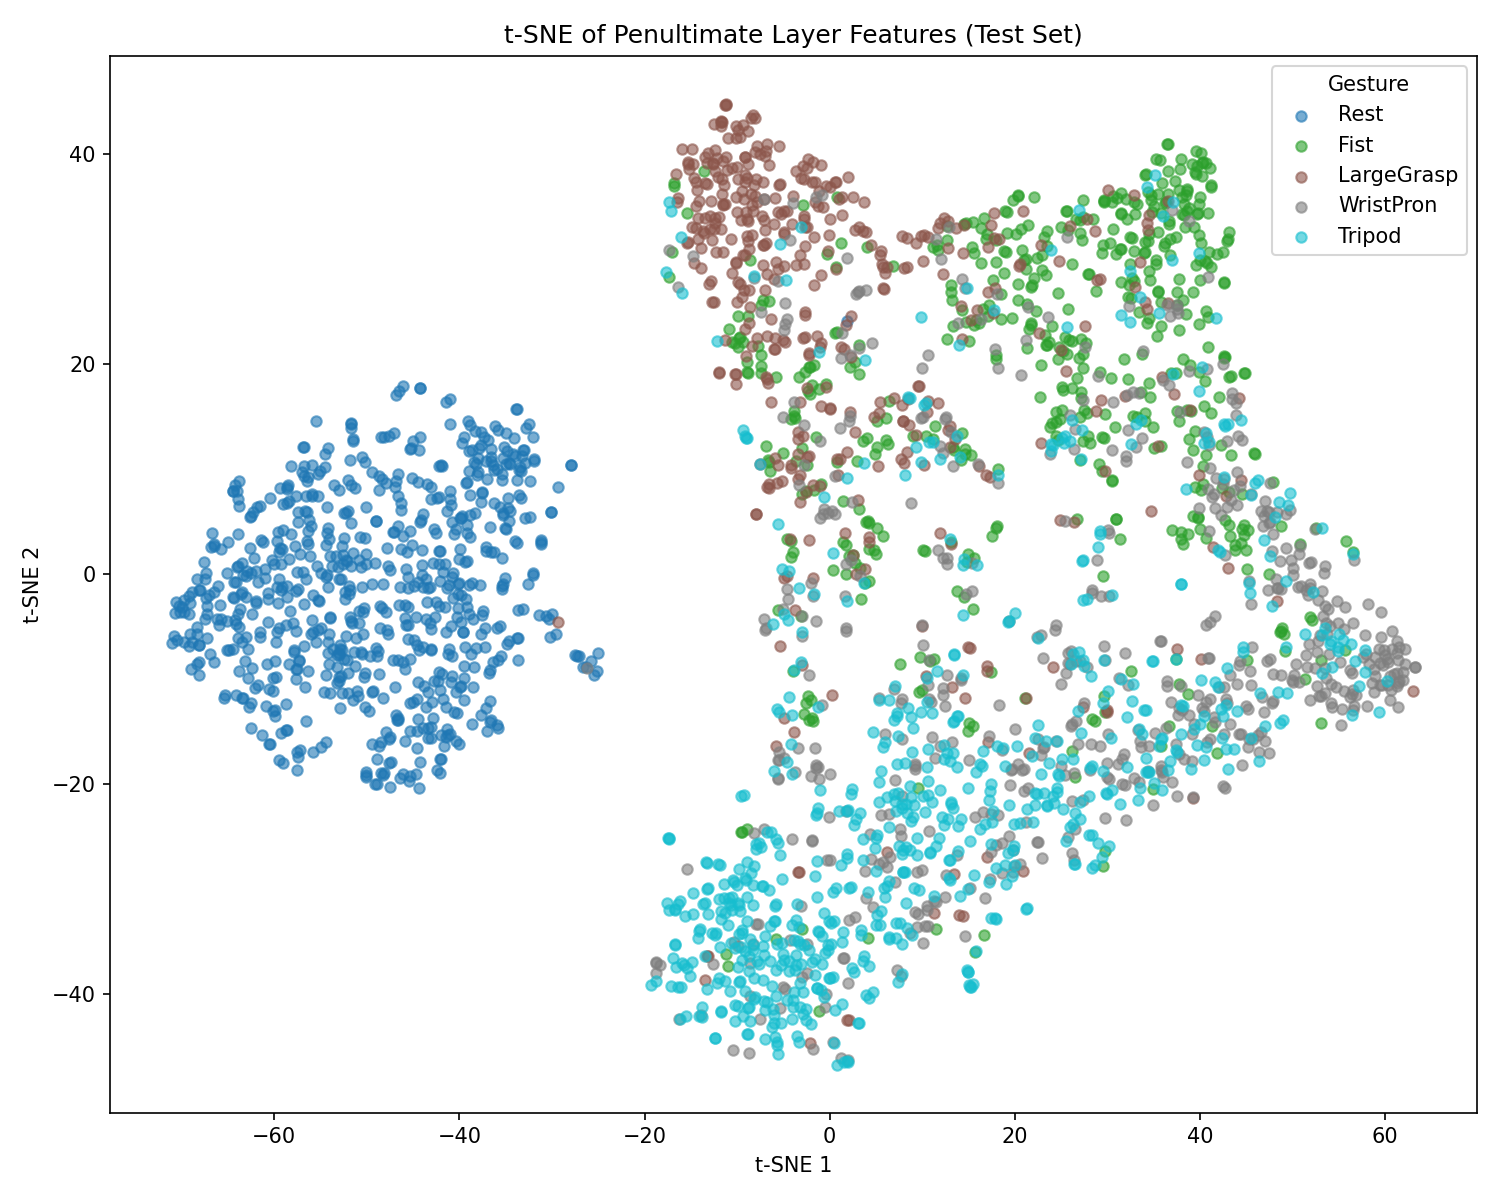
\includegraphics[width=0.95\textwidth]{figures/tsne_features.png}
\caption{t-SNE of penultimate layer features (3,000 test windows).\label{fig:tsne}}
\end{figure}

\subsection{Majority Voting}

The twenty percent improvements (69.87 to 89.78\%) implies the errors are generally independent from each other across the windows of the segment. If the windows have a 0.30 error rate and there are $N=10$ windows, the probability of error falls to 5\%. For Subject 2, these details are illustrated in Figure \ref{fig:voting}.


\begin{figure}[H]
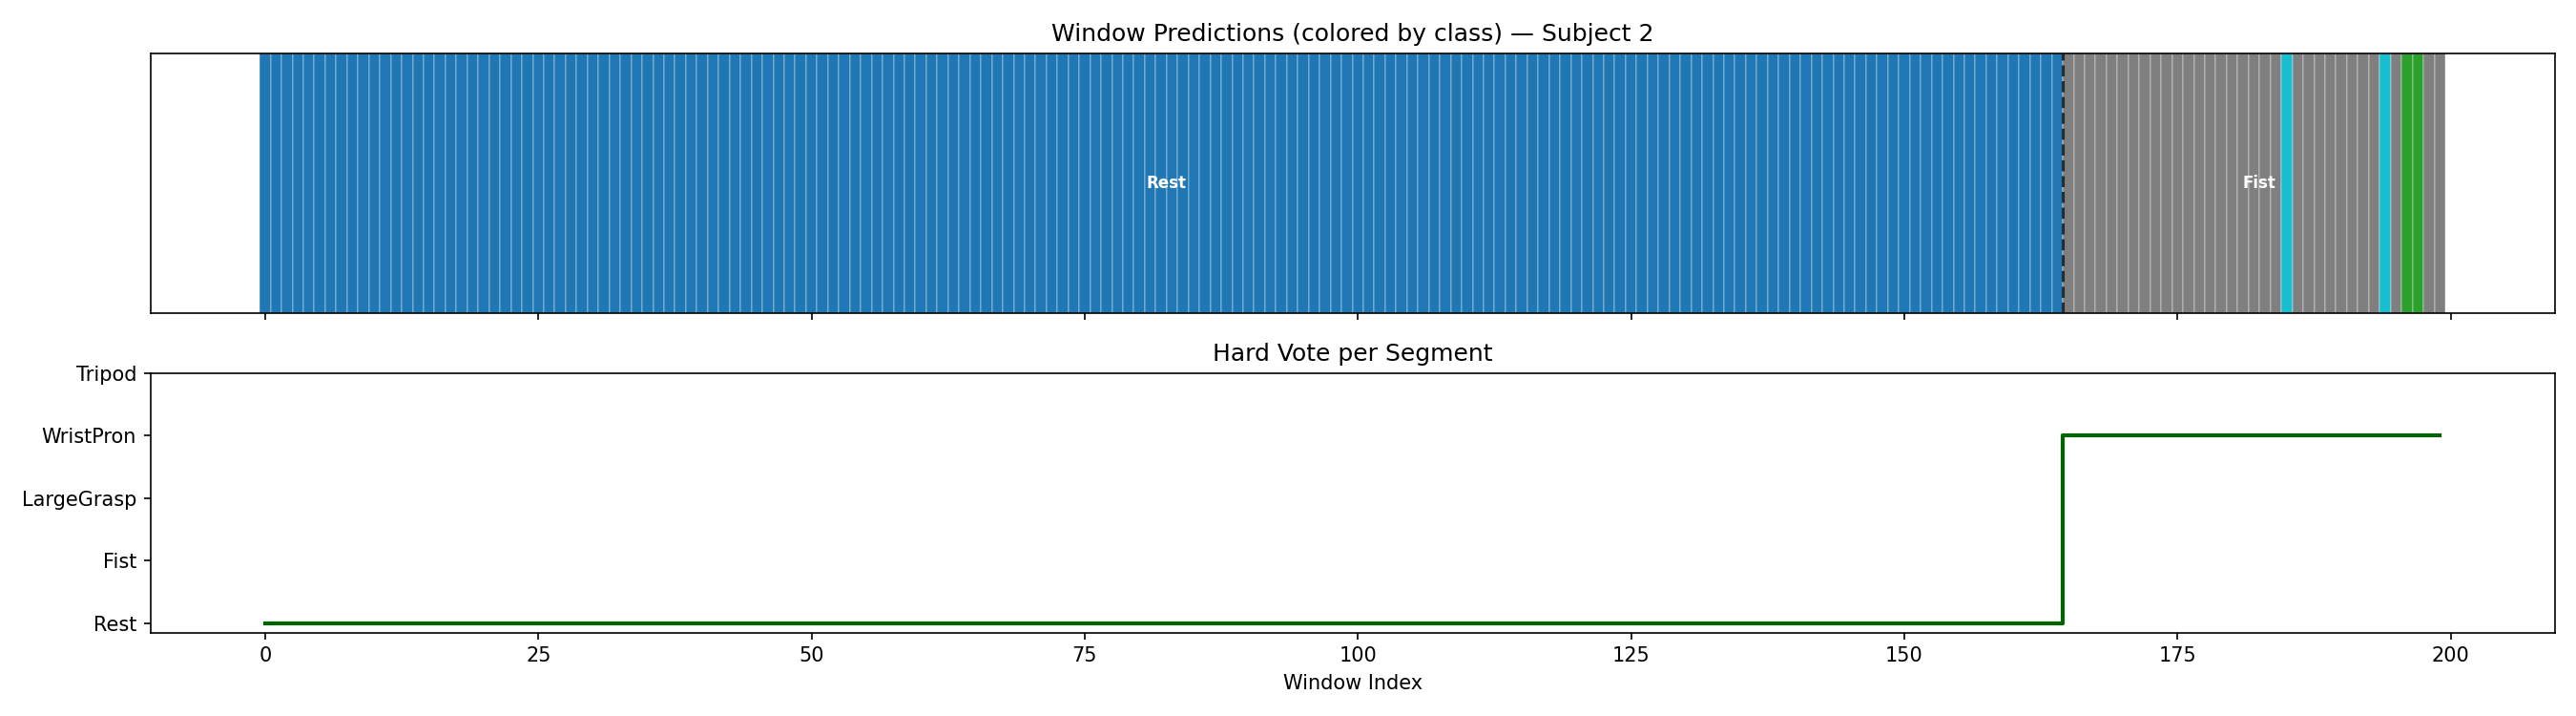
\includegraphics[width= 0.95\textwidth]{figures/voting_segments.png}
\caption{Majority voting illustration for Subject 2.\label{fig:voting}}
\end{figure}

\subsection{Comparison}

Table~\ref{tab:comparison} shows a comparison between our method with two reference approaches. \cite{Lu2023effie} achieved 85\% with (4 gestures), and \cite{Tina2025real} achieved 86.4\% with an (10 gestures).

\begin{table}[H]
\caption{Comparison with reference works.\label{tab:comparison}}
\begin{tabularx}{\textwidth}{lccc}
\toprule
\textbf{Method} & \textbf{Accuracy (\%)} & \textbf{Parameters} & \textbf{Gestures} \\
\midrule
EffiE \citep{Lu2023effie} & 85 & Not reported & 4 \\
Interpretable DL \citep{Tina2025real} & 86.4 & $< 2.5M$ & 10 \\
\textbf{ResCNN + Voting (ours)} & \textbf{89.78} & \textbf{647K} & 5 \\
\bottomrule
\end{tabularx}
\end{table}

It's clear that our segment-level accuracy is competitive, but the different gesture amounts as well as the diverse datasets obstruct the direct comparison between our method and others. The greatest benefit is that there's no further requirement of domain adaptation, meta learning or any fine tuning based on users.


%%%%%%%%%%%%%%%%%%%%%%%%%%%%%%%%%%%%%%%%%%
\section{Conclusions}

This paper goal is to find out weather a simple ResCNN combined by segment level majority voting is capable to predict and recognize sEMG gestures with different subject and limited dataset(e.g. Ninapro DB2) effectively and precise. The ResCNN achieve a window level precision 69.87\%. With using hard majority voting across segments of gesture data, accuracy improved dramatically to 89.78\% (while soft voting achieved a 89.37\% accuracy). This notable improvement of 20 percentage points illustrates that inaccuracies at the window level are largely random within entire gesture segments, thus making a straightforward voting scheme successful in boosting performance. The architectural design introduced, use only 647K trainable parameters, constitutes a robust model that bypasses the requirement for both meta learning and domain adaptation capabilities that often prove out of reach in academia due to limited computing resources and comparatively modest EMG datasets.



%%%%%%%%%%%%%%%%%%%%%%%%%%%%%%%%%%%%%%%%%%
\vspace{6pt}

\dataavailability{The NinaPro DB2 dataset is publicly available at \url{https://ninapro.hevs.ch/}. \\
The code and filtered data subset used in this paper are available ate \url{https://github.com/Mohammed-Alanazii/CS618-Project}.}

%%%%%%%%%%%%%%%%%%%%%%%%%%%%%%%%%%%%%%%%%%

\reftitle{References}

\bibliography{references}


\end{document}
